\documentclass[11pt,a4paper]{article}
\usepackage{fontspec,xeCJK}
\IfFontExistsTF{Microsoft JhengHei}{
  \setCJKmainfont{Microsoft JhengHei}
  \setCJKsansfont{Microsoft JhengHei}
  \setCJKmonofont{Microsoft JhengHei}
}{
  \setCJKmainfont{Noto Serif CJK TC}
  \setCJKsansfont{Noto Sans CJK TC}
  \setCJKmonofont{Noto Sans CJK TC}
}
\usepackage[margin=22mm,headheight=15pt]{geometry}
\usepackage{amsmath,amssymb,graphicx,booktabs,longtable,array,xcolor,hyperref,listings,fancyhdr}
\definecolor{accent}{HTML}{173C57}
\hypersetup{colorlinks=true,linkcolor=accent,urlcolor=accent,pdftitle={DIC02 - CMOS 反相器延遲與負載}}
\setlength{\parindent}{0pt}
\setlength{\parskip}{5pt}
\setlength{\emergencystretch}{3em}
\renewcommand{\arraystretch}{1.2}
\lstset{basicstyle=\ttfamily\small,breaklines=true,columns=fullflexible,frame=single}
\pagestyle{fancy}
\fancyhf{}
\fancyhead[L]{\small DIC02 / 本次模型}
\fancyhead[R]{\small 報告架構預覽}
\fancyfoot[C]{\thepage}
\title{\color{accent}DIC02\\[4pt]CMOS 反相器延遲與負載}
\author{依講義規格重寫之實驗報告}
\date{17 October 2026}
\begin{document}
\maketitle
\begin{center}\small\textbf{中文版・初稿供架構檢視}\\
HSPICE S-2021.09 \quad | \quad 模型庫另行提供
\end{center}
\section{目的}
依 \textit{DIC Lab.pdf} Lab 2（PDF 第 10--12 頁）建立九級 CMOS 反相器鏈，觀察不同輸入上升／下降時間在各級輸出如何轉變，並檢查後級是否接近特徵波形。再分別增加負載至總扇出三，以及將全部反相器寬度放大三倍，重複相同的輸入條件。

本版使用本次模型與 1.0 V 電源，保留講義基本 $W_p/W_n/L=1.8/0.6/0.25\,\mu\mathrm m$。這是製程／電源改寫，不是講義原製程 2.5 V 數據的複製；1.0 V 也不構成對加密模型的額定保證。

\section{Spec 對照}
\begin{center}
\setlength{\tabcolsep}{3pt}
\begin{tabular}{p{0.43\linewidth}p{0.34\linewidth}p{0.17\linewidth}}
\toprule
講義要求（PDF 第 12 頁） & 程式與條件 & 狀態 \\
\midrule
步驟 1：九級鏈、三種輸入邊緣 & \texttt{01\_chain.sp} & 三種均已模擬 \\
觀察 Out1--Out8 的 rise/fall & 每 case 各 16 個 \texttt{.measure} & 72 組 rise/fall 配對 \\
0 ns、0.2 ns、2 $\mu$s & 1 ps 近階躍、0.2 ns、2 $\mu$s & 0 ns 為明示近似 \\
步驟 2：各級總負載三個反相器 & \texttt{02\_fanout3.sp}，主鏈加兩支路 & 三種均已模擬 \\
步驟 3：尺寸加大並重做步驟 1 & \texttt{03\_size3.sp}，全鏈 W 三倍 & 三種均已模擬 \\
\bottomrule
\end{tabular}
\end{center}

三個 deck 各有基本、近階躍、慢邊緣三次分析，共九種情境。Out9 是終端負載，沒有後接同型反相器，因此不以它的無負載 slew 作為特徵波形。講義未指定後級相等的數值誤差門檻；本報告提供量測與差異，沒有另創「必須小於某百分比」的驗收規格。

\section{電路與設計推導}
每級反相器由一顆 PMOS 拉高和一顆 NMOS 拉低，Bulk 分別接電源與地。九級主鏈接法保持不變。FO3 情境在 Out1--Out8 各加入兩個反相器輸入，使總負載為下一級主鏈加兩個支路，並非額外加三個。

尺寸放大情境將全部九級的 $W_n$ 從 0.6 改為 1.8\,$\mu$m、$W_p$ 從 1.8 改為 5.4\,$\mu$m，L 固定為 0.25\,$\mu$m。因驅動與負載同時加大，不能預期輸出時間縮短三倍。用一階估計 $t\sim RC$，若 $R\propto1/W$ 而下一級閘電容 $C\propto W$，兩個效應可大致抵銷。

本實驗測量的是輸出 slew：
\[
\begin{aligned}
t_r&=t(V_o=0.9V_{DD},\uparrow)-t(V_o=0.1V_{DD},\uparrow),\\
t_f&=t(V_o=0.1V_{DD},\downarrow)-t(V_o=0.9V_{DD},\downarrow).
\end{aligned}
\]
它們不是輸入到輸出的 propagation delay。本報告不將 rise/fall time 誤稱為延遲。

\section{模擬設定}
PrimeSim HSPICE S-2021.09 win64、25\,$^\circ$C、\texttt{RUNLVL=6}。一般與近階躍情境的週期為 10 ns、總時間 30 ns；2\,$\mu$s 邊緣情境的週期為 20\,$\mu$s、總時間 60\,$\mu$s。輸入高電位與電源均為 1.0 V，避免原參考程式中 1.8 V 輸入搭配 1 V 電源的不一致。

講義的 0 ns 邊緣用明確的 1 ps 近階躍代替，因為 HSPICE 的零 PULSE 邊緣會採預設時間，不能當成精確零時間。另以 0.1 ps 檢查代表案例的後級敏感度。0.2 ns 與 2\,$\mu$s 兩個條件按原文保留，未將微秒改成奈秒。

\texttt{.tran} 的列印間距在一般情境為 1 ps，慢邊緣情境為 100 ps；求解器採自適應內部步長。列印間距不是保證量測精度的最大步長，故另做 \texttt{RUNLVL=5/6} 敏感度檢查。\texttt{.measure} 將波形的 10\%／90\% 交越轉成數值；\texttt{.tr*} 仍保存波形，\texttt{.mt*} 保存量測表。

HSPICE 亦回報加密區塊的警告遭隱藏；以 \texttt{WARNLIMIT=100} 診斷仍無詳細訊息，因此不宣稱模擬為零警告。診斷量測與原結果一致，但不能據此判定警告無害。

\section{結果與規格檢查}
三個 deck 的九種情境均正常結束，144 個 rise/fall 時間量測均得到數值且未出現失敗標記。以下列出 Out8 的量測以比較輸入條件和負載；逐級完整資料見 \texttt{dic02\_stages.csv}。
\begin{center}
\setlength{\tabcolsep}{3pt}
\begin{tabular}{llrr}
\toprule
配置 & 輸入邊緣 & $t_{r8}$ (ps) & $t_{f8}$ (ps) \\
\midrule
基本 FO1 & 0.2 ns & 134.837 & 77.216 \\
基本 FO1 & 1 ps near-step & 134.766 & 77.187 \\
基本 FO1 & 2 us & 134.817 & 77.233 \\
總扇出 FO3 & 0.2 ns & 323.925 & 217.054 \\
總扇出 FO3 & 1 ps near-step & 323.870 & 216.833 \\
總扇出 FO3 & 2 us & 323.558 & 217.145 \\
全鏈 W 三倍 & 0.2 ns & 134.921 & 76.928 \\
全鏈 W 三倍 & 1 ps near-step & 135.065 & 77.014 \\
全鏈 W 三倍 & 2 us & 134.941 & 76.960 \\
\bottomrule
\end{tabular}
\end{center}
\begin{figure}[htbp]
\centering
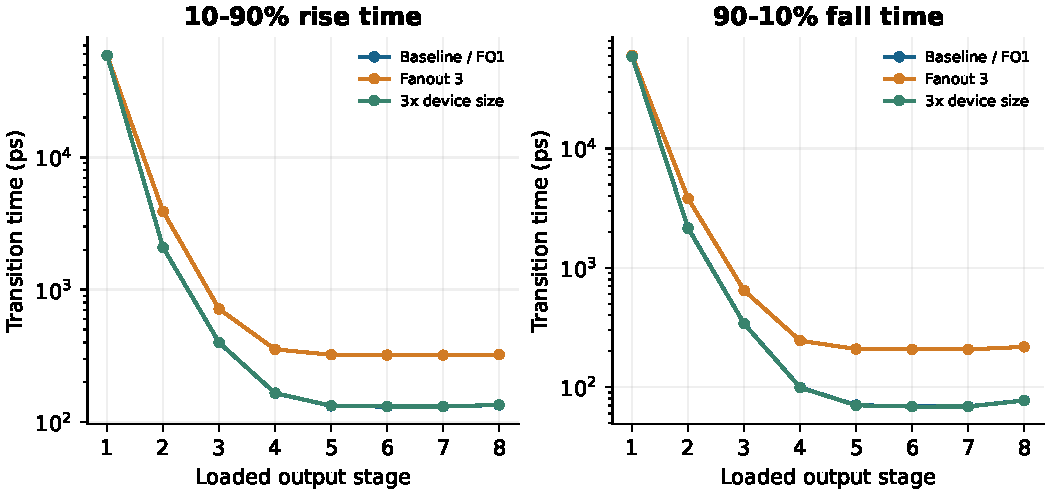
\includegraphics[width=\linewidth]{figures/dic02_stage_evolution.pdf}
\caption{2\,$\mu$s 輸入下 Out1--Out8 的上升與下降時間，依本次 HSPICE 的真實量測表重繪；不是 WaveView 截圖。}
\end{figure}
\begin{figure}[htbp]
\centering
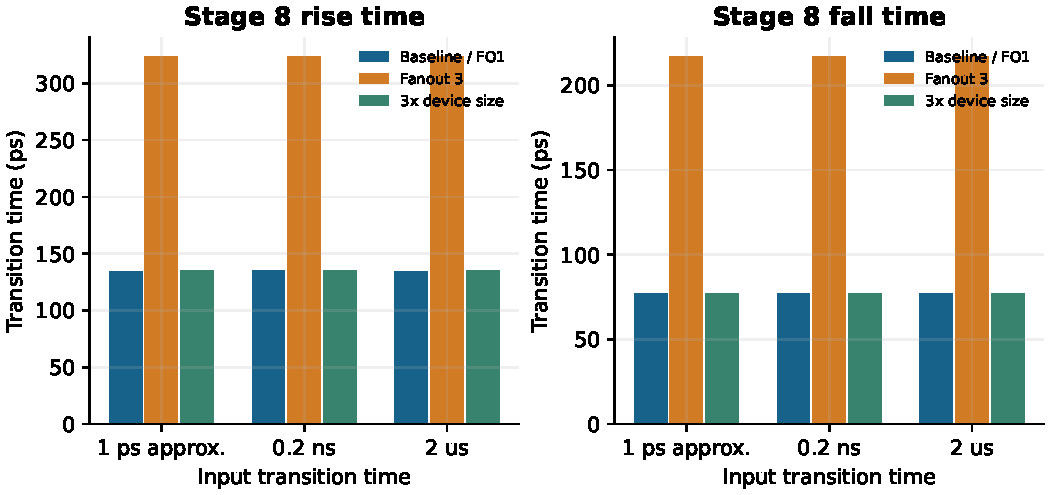
\includegraphics[width=\linewidth]{figures/dic02_stage8.pdf}
\caption{三種鏈配置與三種輸入邊緣的 Out8 實際 rise/fall 量測比較。Out8 仍有終端邊界效應，不以 Out9 無負載輸出取代。}
\end{figure}

基本 FO1 在 2\,$\mu$s 輸入下，Out1 的 $t_r/t_f$ 為 58.881/59.158 ns，Out2 為 2.081/2.160 ns，Out3 為 398.244/340.408 ps。到 Out6 為 130.956/68.551 ps，Out7 為 130.927/68.762 ps，可看到很慢的輸入逐級被整形。

Out8 的 fall time 約 77 ps，與 Out7 約 69 ps 並不完全相同。此差異符合有限九級鏈末端負載的邊界效應解釋：Out9 本身沒有下游負載，其輸出切換會透過輸入電容與 Miller 效應影響 Out8。本次未另做固定 Out9 負載的控制實驗，因此此處屬機理解釋，並非獨立因果驗證。不能據此將所有後級強行視為完全相等。三種初始 slew 對同一配置的 Out8 結果已十分接近，但 rise 與 fall 並不相等。

數值精度檢查發現，預設 \texttt{RUNLVL=3} 對基本鏈的慢輸入前級量測差異很大，故未採用該版結果。最終全部使用 \texttt{RUNLVL=6}。代表性的慢輸入基本鏈，在 \texttt{RUNLVL=5} 與 6 之間，Out1--Out8 全部 rise/fall 的最大相對差為 1.029\%；Out8 rise/fall 分別為 0.1175\%／0.0413\%。近階躍由 1 ps 改為 0.1 ps 時，代表鏈 Out8 rise/fall 的差為 0.0917\%／0.0124\%。這支持本報告後級結論；近階躍的早期尖峰和第一級細節仍可能對邊緣設定敏感，沒有宣稱精確重現 0 ns 的整條波形。

\section{討論}
基本鏈在後級逐漸忘記初始輸入 slew，形成由元件和負載決定的波形；在這組尺寸與本次模型下，拉高和拉低的速度不同，因此 $t_r$ 與 $t_f$ 不必相等。

在 0.2 ns 輸入下，FO3 的 Out8 rise/fall 為 323.925/217.054 ps，明顯慢於 FO1 的 134.837/77.216 ps，符合負載增加的趨勢；不要求倍數精確為三，因為寄生、電壓相關電容與波形都會改變。

全部寬度放大三倍後，Out8 約為 134.921/76.928 ps，與基準接近，證實「放大元件一定使全鏈更快三倍」並不成立。驅動能力提高的同時，下游閘電容也提高。這與只放大驅動器、保持固定外部電容的情境不同。

本次驗證包含電路數量、負載連接、三種輸入條件、完整 Out1--Out8 量測及代表性精度檢查。沒有量到或聲稱滿足講義原製程的特定數字；講義也沒有提供本次模型的容許 slew 誤差或製程 corner 要求。

\section{結論}
九級鏈、總扇出三及全鏈尺寸放大三種配置，均已在三種輸入邊緣下完成實際模擬。數據顯示後級波形趨於穩定、FO3 較慢、全鏈寬度一起放大時 slew 近似不變；有限鏈末端仍有可觀察差異。此結論限於所列模型、1 V、25\,$^\circ$C 條件，並保留 0 ns 的近似處理與原製程不等價的限制。

\end{document}
